\documentclass[letterpaper,11pt]{article}
\usepackage{graphicx}
\usepackage{listings}
\usepackage{hyperref}
\usepackage{amsmath}
\usepackage{url}
\def\UrlBreaks{\do\/\do-}
\usepackage[normalem]{ulem}
\newcommand{\tab}[1]{\hspace{.2\textwidth}\rlap{#1}}
\usepackage{float}
\restylefloat{table}
\usepackage{xcolor}
\usepackage{sectsty}
\sectionfont{\color{blue}}
\usepackage{titlesec}

\titleformat{\section}
{\color{blue}\normalfont\Large\bfseries}
{\color{blue}\thesection}{1em}{}

\lstset{
	basicstyle=\footnotesize,
	breaklines=true,
}

\begin{document}
\begin{titlepage}
\begin{center}


\Huge{Assignment 5}
\newline
\Large{CS595}
\newline
\Large{Introduction to Web Science}
\newline
\Large{Old Dominion University}
\newline
\Large{Computer Science}
\newline
\Large{Due: 11:59 pm Oct 17}
\newline
\Large{Lulwah Alkwai}
\newline
\end{center}
\end{titlepage}
\newpage


The “friendship paradox”: \\
\url{http://en.wikipedia.org/wiki/Friendship_paradox}\\
says that your friends have more friends than you do. 
\section*{ Question One-}

Determine if the friendship paradox holds for your Facebook account. Create a graph of the number of friends (y-axis) and the friends sorted by number of friends (x-axis). \\

(The friends don't need to be labeled on the x-axis.) Do include yourself in the graph and label yourself accordingly. \\

Compute the mean, standard deviation, and median of the number of friends that your friends have. \\

You can download your network in an XML file by using the NameGenWeb Facebook app:  \\
\url{https://apps.facebook.com/namegenweb} \\

You will need to give this app permission to access your Facebook data. Make sure you select "Friend Count" as an Extended Attribute. When you download the data, download it in the GraphML format. \\
If you do not have a Facebook account, email me and I will send you my GraphML file.


\pagebreak
\section*{Answer One-}
Using NameGenWeb I downloaded my Facebook network in an XML file.In my Facebook account I have 64 friends.Where 13 of them have privet accounts (that does not show the number of there friends). So I am left out with 51 friends.

By creating the graph, it shows that almost half of my friends have more friends than me. Because my friends count is 64 and the average is 56; so I am slightly lower than the average. Therefore, I consider the friendship paradox “slightly” holds.


\begin{figure}[!ht]
\centering
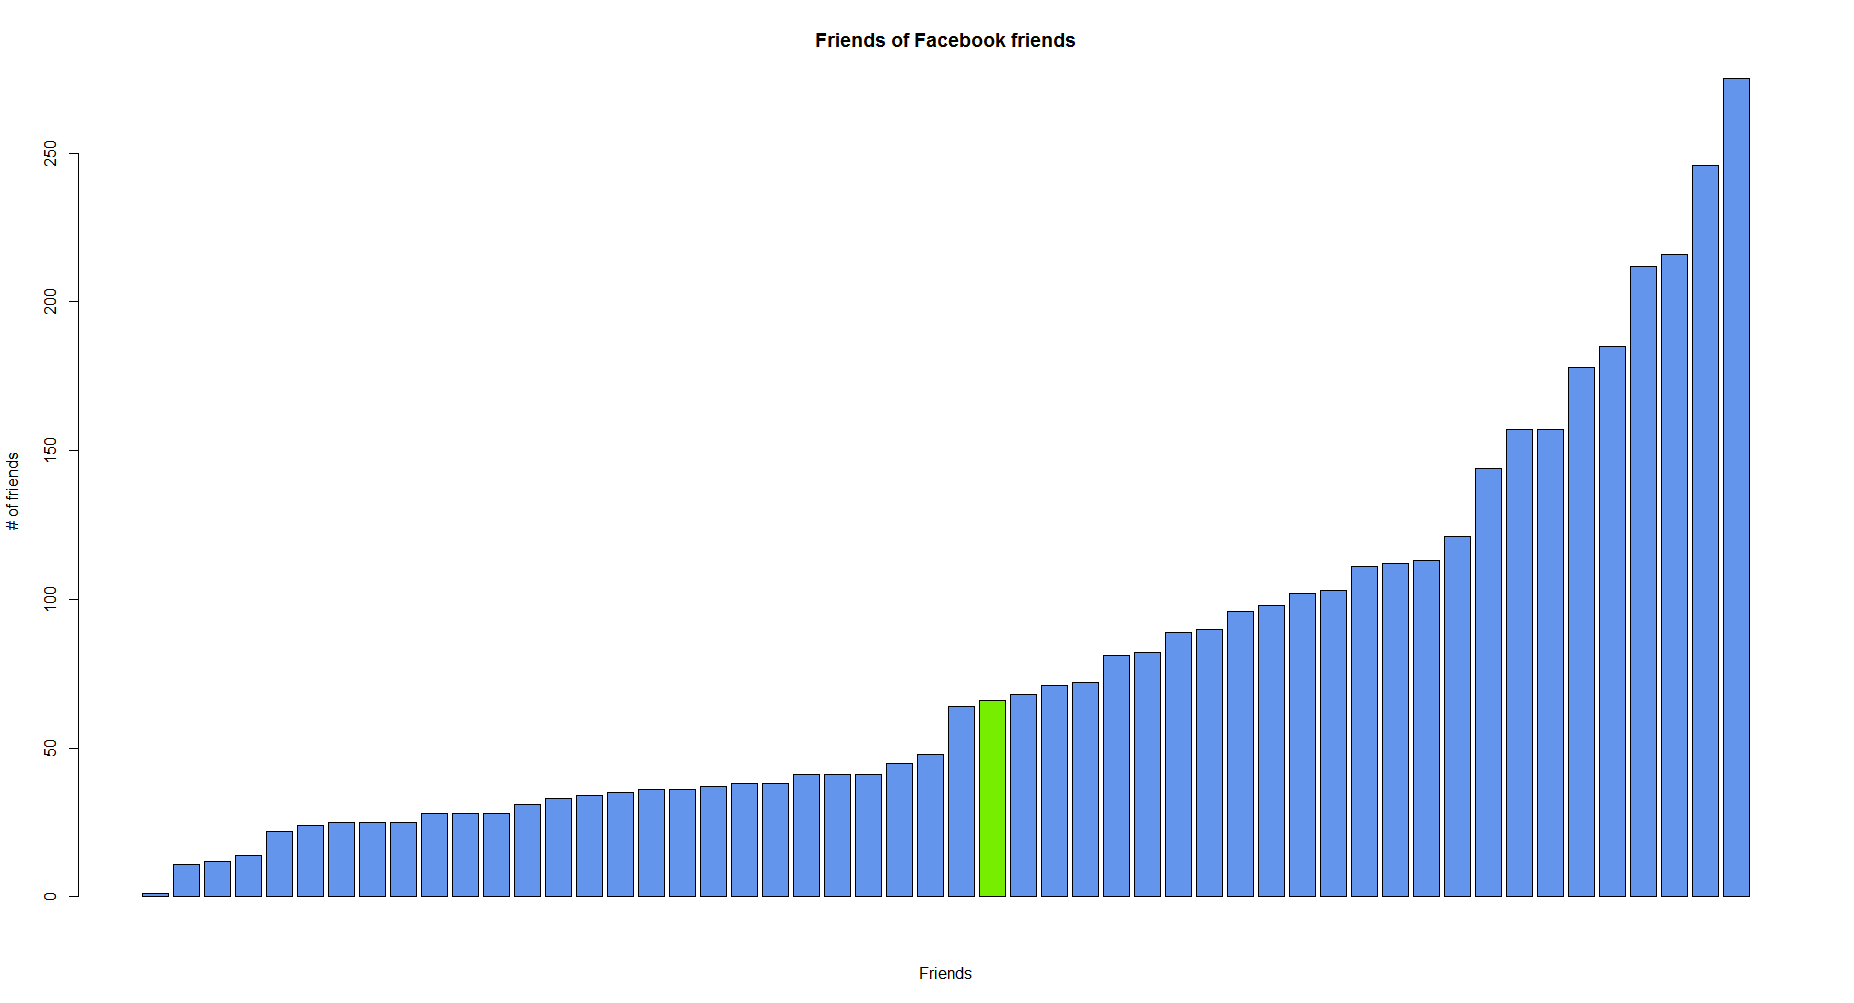
\includegraphics[width=1\textwidth]{1.png}
\caption{Graph for Determining Facebooks Friendship Paradox}
\label{fig:Graph for Determining Friendship Paradox}
\end{figure}


When calculating the Mean, Standard Deviation and the Median I excluded my self and the friends that are private.
\begin{table}[H]
    \begin{tabular}{|| l || l || l ||}\hline
    Mean & Standard Deviation & Median \\\hline
    78.58  & 64.74 & 56 \\\hline
    \end{tabular}
\end{table}
Attached are:
\begin{itemize}
\item (facebooklog.xml): the raw Facebook file obtained.\\
\item (facebookFriends.csv): the processed data
\item (1.png):the Facebook Friends graph.
\ldots
\end{itemize}

\pagebreak
\section*{Question Two-}

Determine if the friendship paradox holds for your Twitter account. Since Twitter is a directed graph, use ``followers'' as value you measure (i.e., ``do your followers have more followers than you?'') \\

Generate the same graph as in question \#1, and calculate the same mean, standard deviation, and median values. \\

For the Twitter 1.1 API to help gather this data, see: \\
\url{https://dev.twitter.com/docs/api/1.1/get/followers/list} \\

If you do not have followers on Twitter (or don't have more than 20), then use my Twitter account ``phonedude\_mln''.

\pagebreak
\section*{Answer Two-}

Using the code on \url{http://thomassileo.com/blog/2013/01/25/using-twitter-rest-api-v1-dot-1-with-python/}\\
I downloaded my Twitter network in an text file. In my Twitter account I have 92 followers. And I took each follower and got the number of their followers. \\

By creating a graph, I had to take the log of the graph since some of the followers have millions of followers, and my data did not show on the graph.\\

The graph showed that most of my followers have more followers than me. So the friendship paradox holds for my Twitter account.

\begin{figure}[!ht]
\centering
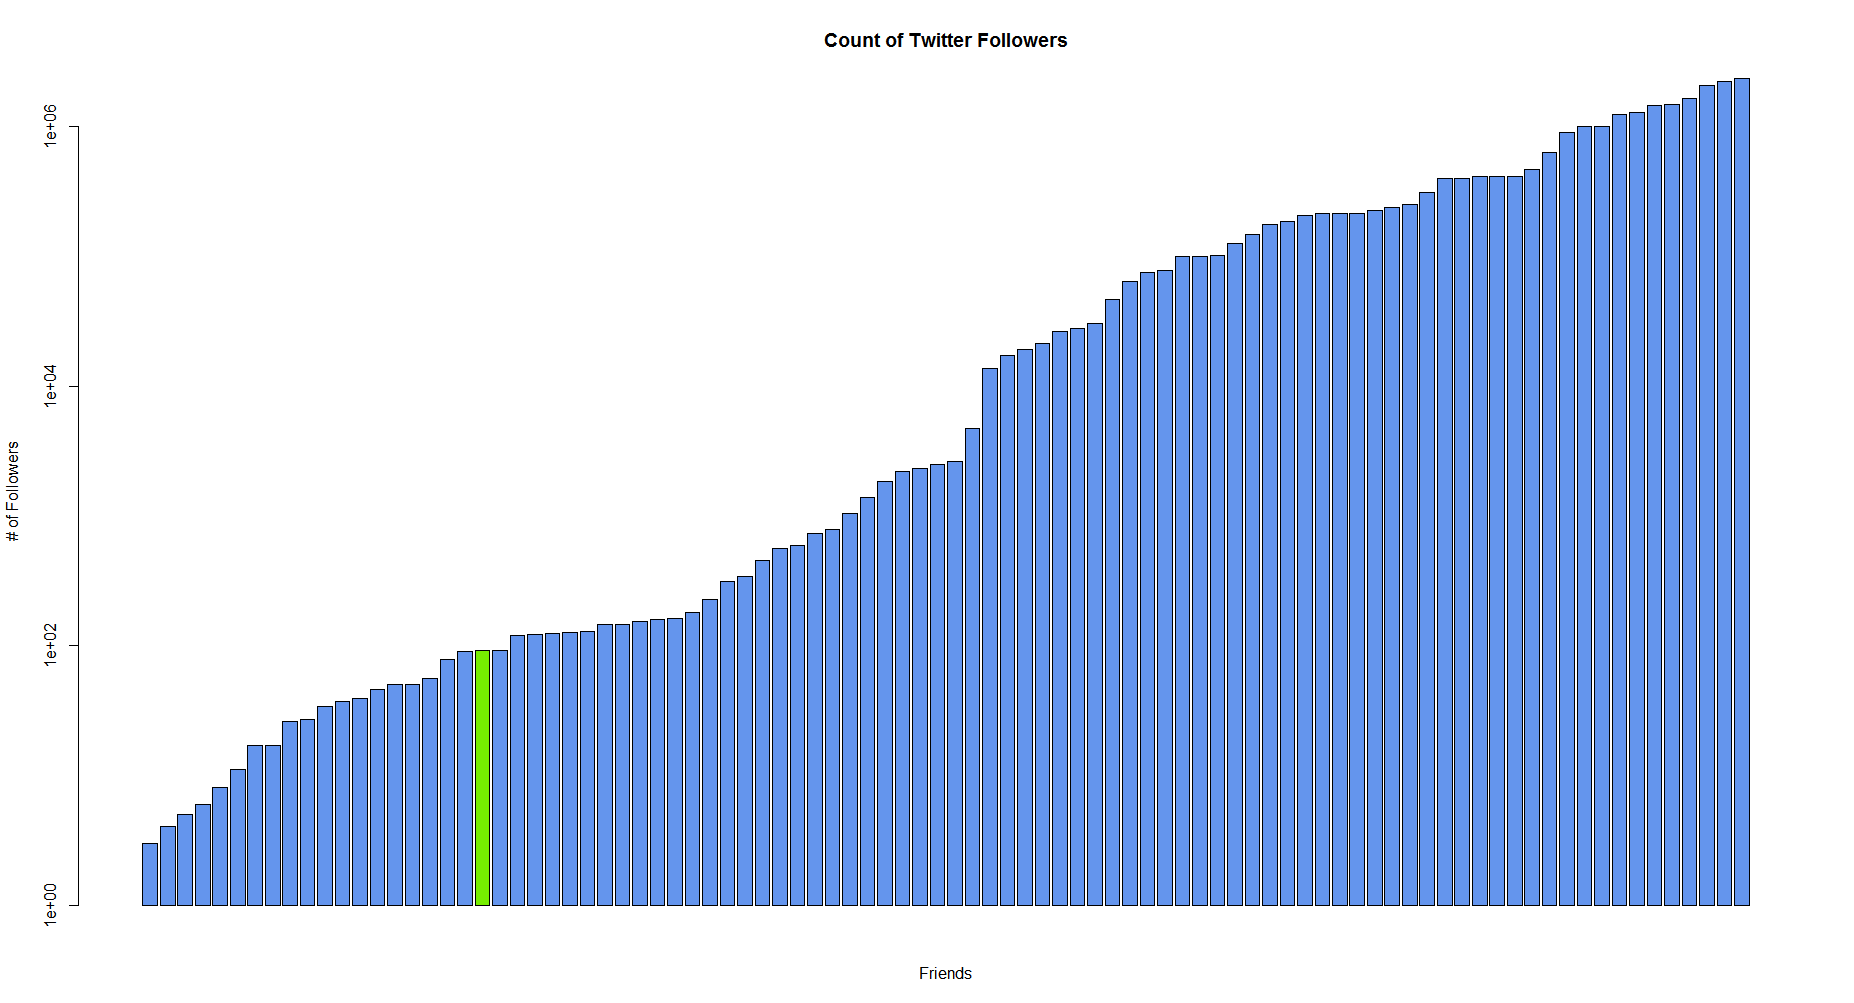
\includegraphics[width=1\textwidth]{2.png}
\caption{Graph for Determining Twitters Friendship Paradox}
\label{fig:Graph for Determining Twitters Friendship Paradox}
\end{figure}


When calculating the Mean,Standard Deviation and the Median I excluded my self.

\begin{table}[H]
    \begin{tabular}{|| l || l || l ||}\hline
    Mean & Standard Deviation & Median \\\hline
    253764.98  & 517076.04 & 2626 \\\hline
    \end{tabular}
\end{table}

Attached are:
\begin{itemize}
\item (a5q2.py): the python code.
\item (twitterlog.txt): the raw twitter file obtained.
\item (twitterFollowers.txt): the processed data.
\item (twitterFollowers.xls): the processed data in excel format.
\item (2.png): the Twitter followers graph.
\ldots
\end{itemize}

\pagebreak
\section*{Question Three-Extra Credit}

Extra credit, 2 points:\\
Repeat question \#1, but with your LinkedIn profile.


\pagebreak
\section*{Answer Three-}
I have created a LinkedIn profile with my name and only found five friends which I requested to link, and since the request is still pending I could not move forward with this question.\\

However, I found this link which states that LinkeIn stopped supporting network statistics.\\
\url{http://help.linkedin.com/app/answers/detail/a_id/220}

\pagebreak
\section*{Question Four-Extra Credit}
Repeat question \#2, but change ``followers'' to ``following''? In other words, are the people I am following following more people?

\pagebreak
\section*{Answer Four-}
Using the same steps as question 2, I used the code on:\\

\url{http://thomassileo.com/blog/2013/01/25/using-twitter-rest-api-v1-dot-1-with-python/}\\

I downloaded my Twitter network in a text file. In my Twitter account I have 381 followings. And I took each following and counted their followings.\\ 

By creating a graph, I had to take the log of the graph since some of the followings have millions of followings, and my data did not show on the graph.\\

The graph showed that most of my followings have more followings than me. So the friendship paradox holds for my Twitter account.


\begin{figure}[!ht]
\centering
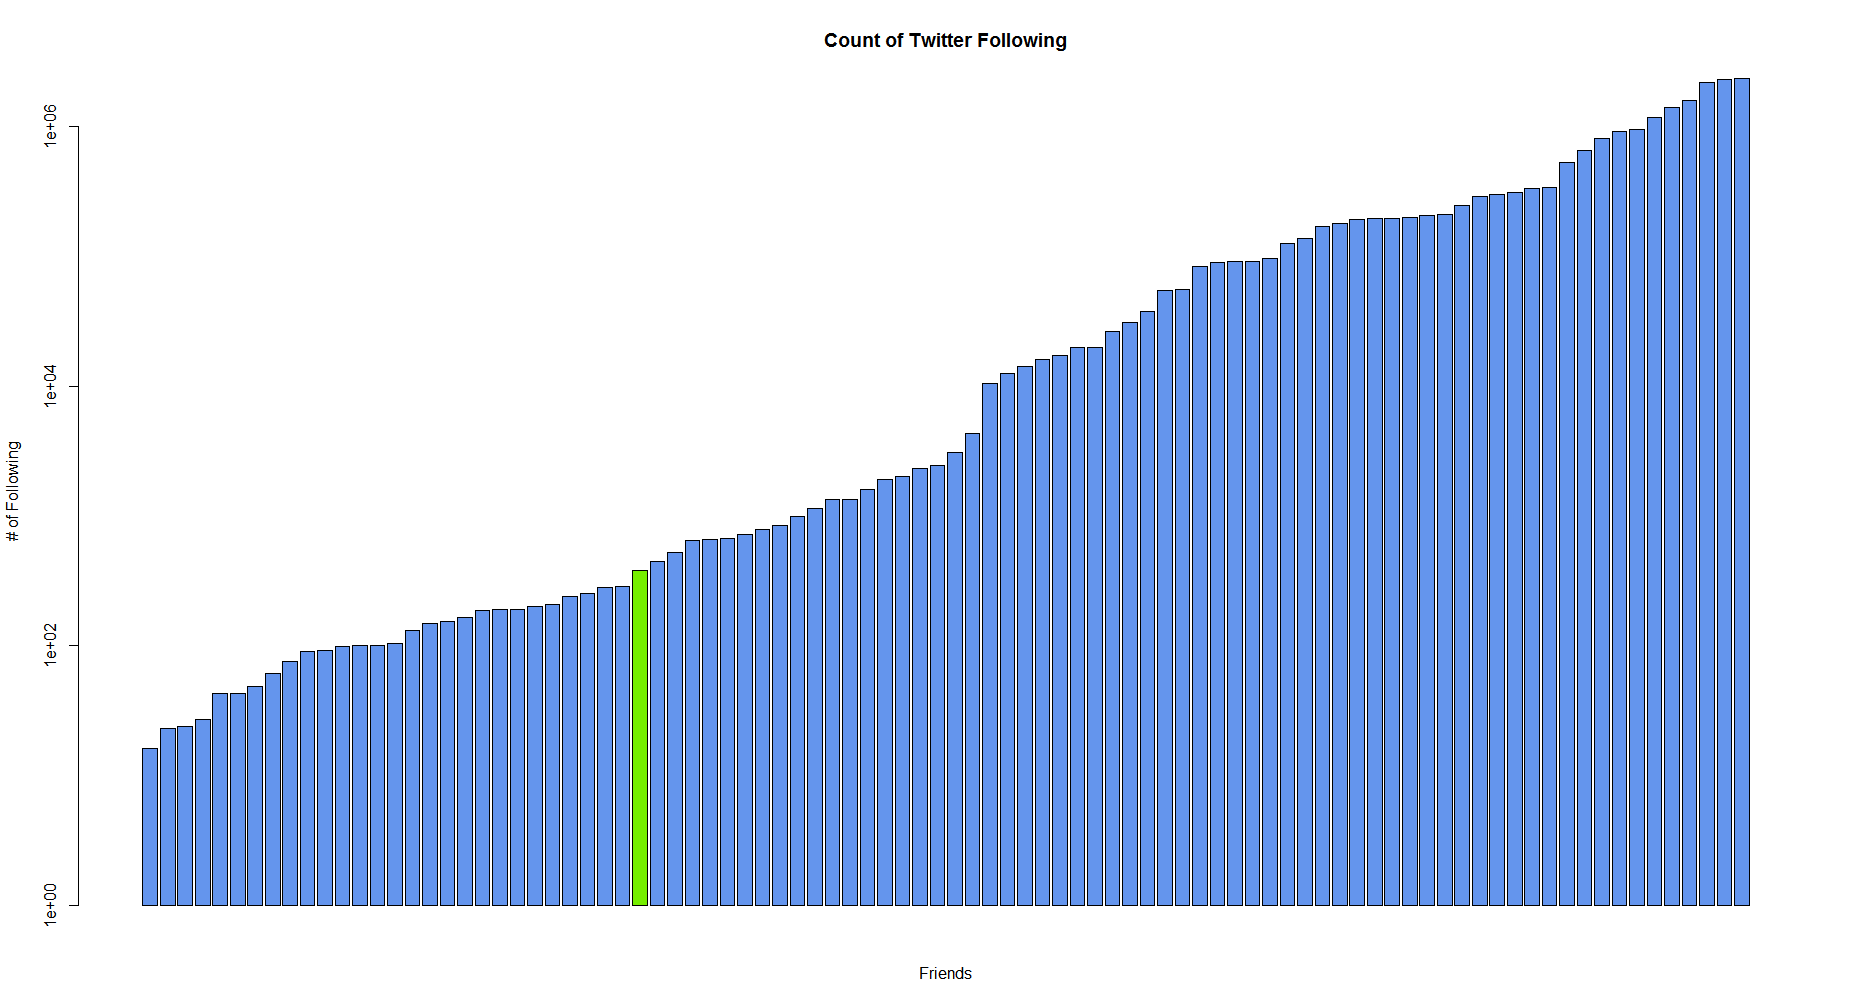
\includegraphics[width=1\textwidth]{4.png}
\caption{Graph for Determining Twitters Friendship Paradox}
\label{fig:Graph for Determining Twitters Friendship Paradox}
\end{figure}


When calculating the Mean,Standard Deviation and the Median I excluded my self.

\begin{table}[H]
    \begin{tabular}{|| l || l || l ||}\hline
    Mean & Standard Deviation & Median \\\hline
    212752.30  & 489936.19 & 3094 \\\hline
    \end{tabular}
\end{table}

Attached are:
\begin{itemize}
\item (a5q4.py): the python code.
\item (twitterlog.txt): the raw twitter file obtained.
\item (twitterFollowings.txt): the processed data.
\item (twitterFollowings.xls): the processed data in excel format.
\item (4.png): the Twitter followers graph.
\ldots
\end{itemize}

\pagebreak
\end{document}